\section{Préliminaires}
Cette section permet d'introduire quelques notions et 
de définir des surfaces qui seront utilisées plus tard 
pour énoncer et démontrer la classification des surfaces.
On fera également des rappels de topologie différentielle. 

\subsection{Variétés et sous-variétés}
On rappelle qu'une variété topologique de dimension $n$ est 
un espace topologique séparé et $\sigma$-compact dont tous 
les points admettent un voisinage ouvert homéomorphe à un ouvert de $\R^n$.

On rappelle également que si $X$ est une variété topologique 
de dimension $n$, une carte est un homéomorphisme d'un ouvert 
de $X$ vers un ouvert de $\R^n$. Un atlas sur $X$ est une famille 
$\lbrace \varphi_i:U_i\to V_i\rbrace$ de cartes sur $X$ telle que 
$\bigcup_iU_i=X$.  Dans un atlas $\mathcal A=\lbrace \varphi_i:U_i\to V_i\rbrace$, 
on appelle changement de carte les applications 
$\varphi_{ij}=\varphi_j\circ\varphi_i^{-1}:\varphi_i(U_i\cap U_j)\to \varphi_j(U_i\cap U_j)$.
Un atlas est lisse lorsque tous ses changements de cartes sont lisses. 
Deux atlas lisses sont équivalents si leur réunion est encore un atlas lisse.

\begin{defi}
    Une variété différentielle (de classe $\mathcal C^\infty$) est la donnée 
    d'une paire $(X,\Sigma)$ où $X$ est une variété topologique et où $\Sigma$ 
    est une classe d'équivalence d'atlas lisses sur $X$.
\end{defi}

On parle ainsi de \textit{structure} de variété différentielle. 
Comme pour les groupes ou autre structures algébriques, on pourra 
parler d'une "variété différentielle $X$" au lieu de "variété différentielle $(X,\Sigma)$", 
la structure étant la plupart du temps sous-entendue dans les notations.
Dans toute la suite, le mot "variété" désignera une variété différentielle 
de classe $\mathcal C^\infty$.  Une surface sera alors une variété de 
dimension $2$. Des exemples de surfaces (et donc de variétés) sont la 
sphère $\mathbb S^2$, le tore $\mathbb T^2$, le ruban de Möbius, la bouteille de Klein... 

\begin{center}
    \begin{tikzpicture}[scale=.4]
    % Boule
    \shade[ball color=gray!90,opacity = 0.2] (0,0) circle (4cm);
	\draw[thick] (0,0) circle (4cm);
	\draw[thick] (-4,0) arc (180:360:4 and 0.6);
	\draw[thick,dashed] (4,0) arc (0:180:4 and 0.6);
    %% Ouvert Ui
    \node (p1) at (-2.5, -0.4) {};
    \node (p2) at (-0.5, 2.0) {};
    \node (p3) at (0.4, 0.1) {};
    \path[fill,AccColor1!50,opacity=0.5]plot [smooth cycle,tension=1] coordinates {(p1) (p2) (p3)};
    \node at (-1.8, 2.0) {$U_i$};
    % Ouvert Uj
    \node (q1) at (-0.5,0) {};
    \node (q2) at (2.0,-1) {};
    \node (q3) at (2.0, 0.5) {};
    \node (q4) at (-0.5, 1.0) {};
    \path[fill,AccColor2!50,opacity=0.5]plot [smooth cycle,tension=1] coordinates {(q1) (q2) (q3)(q4)};
    \path[thick,draw,black]plot [smooth cycle,tension=1] coordinates {(q1) (q2) (q3)(q4)};
    \path[thick,draw,black]plot [smooth cycle,tension=1] coordinates {(p1) (p2) (p3)}; 
	\node at (2,1.1) {$U_j$};

    % Ouvert d'arrivée i
    \node (p1) at (8, 2) {};
    \node (p2) at (12.5, 5.0) {};
    \node (p3) at (12.4, 2.1) {};
    \path[fill,AccColor1!30]plot [smooth cycle,tension=1] coordinates {(p1) (p2) (p3)};
    \path[thick,draw,black]plot [smooth cycle,tension=1] coordinates {(p1) (p2) (p3)}; 
	\node at (10.5,2.8) {$\varphi_i(U_i)$};
    
    % Ouvert d'arrivée j
    \node (q1) at (8.0,-5) {};
    \node (q2) at (12.5,-5.2) {};
    \node (q3) at (12.5, -2.3) {};
    \node (q4) at (8.3, -2.3) {};
    \path[fill,AccColor2!30]plot [smooth cycle,tension=1] coordinates {(q1) (q2) (q3)(q4)};
    \path[thick, draw, black]plot [smooth cycle,tension=1] coordinates {(q1) (q2) (q3)(q4)};
    \node at (10.5,-3.7) {$\varphi_j(U_j)$};

    % Flèche changement de carte
	\node at (16.2,3) {$\varphi_i (U_i \cap U_j)$};
	\draw [very thick, arrow] (16.2,-3) to (16.2,2) ;
	\node at (16.2,-4.2) {$\varphi_j (U_i \cap U_j)$};
	\node at (15.5,-0.5) [left] {$\varphi_{ij}$};

    % Flèches cartes
	\draw [very thick,arrow,bend angle=45,bend left]  (-0.2,1.2)  to (8.4,3) ;
	\node at (5,4.7) {$\varphi_i$};
	\draw [very thick,arrow,bend angle=45,bend right]  (0.5,0)  to (7.5,-5) ;
	\node at (5,-4.2) {$\varphi_j$};
\end{tikzpicture}\\
    \vspace{1em}
    \textsc{Figure 1} – \textit{Changements de cartes}
\end{center}

\begin{defi}
    Une partie $Y$ d'une variété $X$ de dimension $n$ est une sous-variété 
    de codimension $k\leq n$ si tout point de $Y$ est contenu dans le domaine 
    d'une carte $\varphi:U\hookrightarrow\R^n$ vérifiant 
    \[
        \varphi(Y\cap U)=\varphi(U)\times(\R^{n-k}\times\lbrace 0\rbrace)
    \]
\end{defi}

On voit très facilement qu'il est possible de munir une sous-variété $Y$ 
d'une structure de variété, simplement par restriction des cartes sur $X$.

\begin{remark}
    On retrouve bien la définition de sous-variété de $\R^n$ vue dans le cours 
    de calcul différentiel de L3, en choisissant le bon atlas lisse sur $\R^n$.
\end{remark}

\subsection{Applications différentiables sur des variétés}

\begin{defi}
    Soit $f:M\to N$ une application entre deux variétés de dimensions $n$ et 
    $p$ respectivement. Soit $x\in M$. On dit que $f$ est différentiable 
    (resp. lisse) en $x$ s'il existe des cartes $\varphi:U\to \R^n$ et $\psi:V\to\R^p$
    autour de $x$ et $f(x)$ respectivement telles que $\psi\circ f\circ\varphi^{-1}$ 
    est différentiable (resp. $\mathcal C^\infty$) en $\varphi(x)$.
\end{defi}

En particulier, une fonction $f:S\to \R$ partant d'une surface $S$ est lisse si 
pour toute carte $\varphi:U\to\R^2$, $f\circ\varphi^{-1}$ est lisse. Sauf mention 
du contraire, toutes les applications entre variétés seront supposées lisses dans 
la suite du document.

\begin{center}
    \begin{tikzpicture}[scale=.5]
    % Boule 1
    %% Boule
    \shade[ball color = gray!90, opacity = 0.2] (0,0) circle (4cm);
	\draw[thick] (0,0) circle (4cm);
	\draw[thick, rotate=30] (-4,0) arc (180:360:4 and 1);
    \draw[thick, rotate=30] (0,-4) arc (270:90:1 and 4);
    \node at (0,4.2) [above] {$M$};
    %% Ouvert U dans la boule 1
    \node (q1) at (-.5,.5) {};
    \node (q2) at (1.5,.5) {};
    \node (q3) at (1.7, 2) {};
    \node (q4) at (0, 3) {};
    \path[fill,AccColor1!50] plot [smooth cycle,tension=1] coordinates {(q1) (q2) (q3) (q4)};
    \path[thick, draw, black]plot [smooth cycle,tension=1] coordinates {(q1) (q2) (q3) (q4)};
	\node at (.5,1.4) {$U$};

    % Boule 2
    %% Boule 
    \shade[ball color = gray!90, opacity = 0.2] (15,0) circle (4cm);
	\draw[thick] (15,0) circle (4cm);
	\draw[thick] (11,0) arc (180:360:4 and 1);
    \draw[thick] (15,-4) arc (270:90:1 and 4);
    \node at (15,4.2) [above] {$N$};
    %% Ouvert V dans la boule 2
    \node (q1) at (11.8,.5) {};
    \node (q2) at (13.3,.5) {};
    \node (q3) at (13.5, 2) {};
    \node (q4) at (12.5, 1.9) {};
    \path[fill,AccColor2!50] plot [smooth cycle,tension=1] coordinates {(q1) (q2) (q3) (q4)};
    \path[thick,draw,black]plot [smooth cycle,tension=1] coordinates {(q1) (q2) (q3) (q4)};
	\node at (12.8, 1.1) {$V$};

    % Flèches
	\draw[very thick, arrow, bend angle=10, bend left] (3.5,3.5) to (11.5,3.5);
	\node at (7.5,4) [above] {$f$};
    \draw[very thick, arrow] (0,-4) to (0,-7);
    \node at (0,-5.5) [left] {$\varphi$};
    \draw[very thick, arrow] (15,-4) to (15,-7);
    \node at (15,-5.5) [right] {$\psi$};
    \draw[very thick, arrow, bend angle=10, bend left] (2,-7) to (12.5,-7);
    \node at (7.25,-6.5) [above] {$\psi\circ f\circ\varphi^{-1}$};

    % Blob Rn
    \node (q1) at (-1,-7) {};
    \node (q2) at (.8,-7.1) {};
    \node (q3) at (.7,-8.3) {};
    \node (q4) at (-1.3,-8.4) {};
    \path[draw,thick,black] plot [smooth cycle,tension=1] coordinates {(q1) (q2) (q3) (q4)};
    \node at (-1.3,-7) [left] {$\R^n$};

    % Blob Rp
    \node (q1) at (14,-7) {};
    \node (q2) at (15.8,-7.1) {};
    \node (q3) at (15.7,-8.3) {};
    \node (q4) at (13.6,-8.2) {};
    \path[draw,thick,black] plot [smooth cycle,tension=1] coordinates {(q1) (q2) (q3) (q4)};
    \node at (16,-7) [right] {$\R^p$};

% Menge 1 auf Kugel
    % \node (p1) at (8, 2) {};
    % \node (p2) at (12.5, 5.0) {};
    % \node (p3) at (12.4, 2.1) {};
    % \path plot [smooth cycle,tension=1] coordinates {(p1) (p2) (p3)};
    % \path[thick, draw, black] plot [smooth cycle,tension=1] coordinates {(p1) (p2) (p3)}; 
	% \node at (10.5,2.8)   {$V_\alpha$};
    
% Menge 2 auf Kugel
    % \node (q1) at (8.0,-5) {};
    % \node (q2) at (12.5,-5.2) {};
    % \node (q3) at (12.5, -2.3) {};
    % \node (q4) at (8.3, -2.3) {};
    %\begin{pgfonlayer}{background}
    %\path plot [smooth cycle,tension=1] coordinates {(q1) (q2) (q3)(q4)};
    %path[thick, draw, black]plot [smooth cycle,tension=1] coordinates {(q1) (q2) (q3)(q4)};
    %\node at (10.5,-3.7)   {$V_\beta$};

% Kartenwechsel
	% \node at (16,3)   {$x_\alpha (U_\alpha \cap U_\beta)$};
	% \draw [very thick, arrow]  (16,-3)  to (16,2) ;
	% \node at (16,-4.2)   {$x_\beta (U_\alpha \cap U_\beta)$};
	% \node at (14,-0.5)   {$x_\alpha \circ x^{-1}_\beta$};      
\end{tikzpicture}

	
    \textsc{Figure 2} – \textit{Application différentiable entre variétés}
\end{center}

Nous allons à présent définir les notions d'immersion, submersion, plongement et de 
difféomorphisme entre deux variétés. 

\begin{defi}
    Une application $f:X\to Y$ différentiable entre deux variétés de dimensions $n$ 
    et $p$ respectivement est appelée 
    \begin{enumerate}[(i)]
        \item une immersion si son rang vaut partout $n$;
        \item une submersion si son rang vaut partout $p$;
        \item un difféomorphisme local si son rang vaut partout $n$ et $p$.
    \end{enumerate}
    Un difféomorphisme entre deux variétés est une application lisse bijective dont 
    la réciproque est aussi lisse.  Un plongement d'une variété $N$ dans une variété 
    $M$ est une immersion $f$ qui est un homéomorphisme sur son image. 
\end{defi}

Ainsi, lorsqu'il existe un difféomorphisme entre deux variétés, on dira qu'elles sont 
difféomorphisme.

Le but, comme énoncé en introduction, est de classifier, à homéomorphisme près, les 
surfaces connexes, compactes et orientables (la notion d'orientable sera définie un 
peu plus bas). Par ailleurs, dans toute la suite, le mot "surface" désignera une surface 
connexe, compacte et orientable.

\begin{defi}
    Soient $f_0,f_1:M\to M$ des difféomorphismes où $M$ est une variété.
    Les applications $f_i$ sont dites homotopes s'il existe une application lisse 
    (une homotopie lisse) $F:[0,1]\times M\to M$ telle que 
    \begin{enumerate}[(i)]
        \item $\forall x\in M, F(0,x)=f_1(x)$;
        \item $\forall x\in M, F(1,x)=f_2(x)$;
        \item Pour tout $t\in[0,1]$, l'application $F(t,\cdot)$ est un difféomorphisme.
    \end{enumerate}
\end{defi}

\subsection{Fibré tangent, champ de vecteurs et groupe à paramètre}
\begin{defi}
    On considère $M$ une variété et $x\in M$. On note $C_xM$ l'ensemble des courbes 
    lisses passant par $x$ en $0$.
    On dit que deux éléments $\gamma_0$ et $\gamma_1$ de $C_xM$ ont même vitesse en 
    $0$ s'il existe une carte $\varphi:V\to\R^n$ telle que $V$ contient $x$ et 
    $\varphi\circ\gamma_0$ et $\varphi\circ\gamma_1$ ont même dérivée en $0$.
    Ainsi, l'espace tangent $T_xM$ de $M$ en $x$ est le quotient de $C_xM$ par la 
    relation d'équivalence "avoir la même vitesse en $0$". 
    On définit l'ensemble $TM$, réunion disjointe des $\lbrace p\rbrace\times T_pM$ 
    pour $p\in M$, que l'on appelle fibré tangent.
\end{defi}

\begin{remarks}
    \begin{itemize}
        \item Les espaces tangents $T_xM$ peuvent être munis d'une structure d'espace 
        vectoriel, leur dimension étant celle de la variété $M$ ;
        \item Le fibré tangent $TM$ peut-être muni d'une structure de variété, sa 
        dimension est égale à deux fois celle de $M$.
    \end{itemize}
\end{remarks}

\begin{center}
    \begin{tikzpicture}[x=0.75pt, y=0.75pt, yscale=-1, scale=.75]
    height of 300
  
    % The manifold
    \draw[thick] (112.04,66.62) node[above right, font=\scriptsize]{$M$};
    \draw[thick] (100,108) .. controls (140,78) and (188,143) 
                    .. (196,182) ;
    \draw[thick] (196.2,181.8) .. controls (211.8,159.6) and (265.71,101.03) 
                        .. (318.8,111.8) ;
    \draw[thick] (318.8,111.8) .. controls (323.67,112.42) and (330.33,115.42) 
                        .. (335,118) ;
    \draw[dotted] (219.48,53.8) .. controls (230.71,56.06) and (244.01,58.07) 
                                .. (259,63.39) ;
    \draw[thick] (259,63.39) .. controls (288.81,75.27) and (332.14,114.93) 
                      .. (335,118) ;
    \draw[thick] (100,108) .. controls (113.56,84.56) and (160.04,48.06) 
                    .. (219.48,53.8) ;
  
    % The tangent space at x
    \draw[thick] (238.68,46.2) -- (294.01,93.72) 
                        -- (224.01,122.72) 
                        -- (168.68,75.2) 
                        -- cycle ;
    \fill[AccColor2!40,opacity=.5] (238.68,46.2) -- (294.01,93.72) 
                        -- (224.01,122.72) 
                        -- (168.68,75.2) 
                        -- cycle ;                        
    \draw (173.51,76.9) node[below right, 
                             font=\scriptsize, 
                             rotate=-337.86,
                             xslant=-0.54]{$T_{x} M$};

    % A point x in the manifold
    \filldraw (232.9,84.2) circle (1pt)
    node[below right, font=\scriptsize]{$x$};
  \end{tikzpicture}\\
    \vspace{1em}
    \textsc{Figure 3} – \textit{Espace tangent en $x$}
\end{center}

Lorsque $M$ et $N$ sont des variétés et que $f:M\to N$ est une application lisse, 
cette dernière induit une application $C_xf:C_xM\to C_{f(x)}N$ pour $x\in M$ qui 
envoie $\gamma$ sur $f\circ \gamma$.

\begin{defi}
    L'application tangente à $f:M\to N$ en un point $x$ est l'application 
    $T_xf:T_xM\to T_{f(x)}N$ induite par $C_xf$.
    On définit $Tf:TM\to TN$ par $Tf(x,v)=(f(x),T_xf(v))$, aussi notée $\dd f$ ou $f_*$.
\end{defi}

À présent, on définit la notion de champ de vecteurs sur une variété.

\begin{defi}
    Un champ de vecteurs sur une variété $M$ est une application $X:M\to TM$
    telle que pour tout $x\in M$, $X(x)\in\lbrace x\rbrace\times T_xM$.
\end{defi}
Comme mentionné dans une précédente remarque, $TM$ est une variété, on peut alors 
parler de champ de vecteurs \textit{lisse}.

\begin{defi}
    Un groupe de paramètre de difféomorphismes d'une variété $M$ est une application 
    $\varphi:\R\times M\to M$ telle que 
    \begin{enumerate}[(i)]
        \item pour tout $t\in\R$, l'application $\varphi_t=\varphi(t,\cdot):M\to M$ est 
        un difféomorphisme ;
        \item pour tous $s$ et $t$, on a $\varphi_{s+t}=\varphi_t\circ\varphi_s$, en 
        particulier $\varphi_0=\id_M$.
    \end{enumerate}
\end{defi}

Étant donné $\varphi$ un groupe à paramètre de difféomorphismes, on définit un champ de 
vecteurs $X$ comme suit : au point $x\in M$, on pose 

\[
    X(x)=\partial_t\varphi(\cdot,x)(0)
\]

$X(x)$ est la vitesse en $0$ du chemin $t\mapsto\varphi_t(x)$.
On peut remarquer que $\partial_t\varphi(\cdot,x)(s)=X(\varphi_s(x))$ en utilisant le point 
(ii) de la définition.

On dit que $X$ engendre le groupe à paramètre de difféomorphismes $\varphi$.

\begin{prop}
    Soit $M$ une variété et $X$ un champ de vecteurs sur $M$, lisse et nul en dehors d'un 
    compact. 
    Alors, il existe un unique groupe à paramètre de difféomorphismes engendré par $X$.
\end{prop}

\begin{proof}
    On construit d'abord un groupe à paramètre de difféomorphismes engendré par $X$. 
    Soit $K$ un compact vérifiant l'hypothèse de l'énoncé. 
    En tout point $p$ du compact, on sait trouver un voisinage ouvert $U_p$ de $p$ ainsi qu'un 
    réel $\varepsilon(p)>0$ tel qu'il existe une unique solution au problème de Cauchy
    \[
        \left\lbrace\begin{array}{c} y' = X(y)\\ y(0)=x\end{array}\right.
    \]
    définie sur $(-\varepsilon(p),\varepsilon(p))$ pour tout $x\in U_p$, que l'on va noter 
    $\varphi_t(x)$.
    La famille d'ouverts $(U_p)_{p\in K}$ recouvre le compact $K$, on sait alors en extraire 
    une famille finie $(U_{p_1},\dots,U_{p_\alpha})$ recouvrant $K$, et on prend alors 
    $\varepsilon$ le plus petit des réels $\varepsilon(p_1),\dots,\varepsilon(p_\alpha)$.
    Ainsi, $\varphi_t(x)$ est bien défini en tout $(t,x)\in(-\varepsilon,\varepsilon)\times K$. 
    Si $x\notin K$, on pose $\varphi_t(x)=x$ pour tout $t\in\R$, un résultat de théorie des 
    équations différentielles ordinaires permet d'assurer qu'à ce stade, $\varphi$ est une 
    fonction lisse des deux variables.
    En dérivant $\varphi(\cdot+s,x)$ pour un $s$ fixé, on montre facilement que, pourvu que 
    $|t+s|<\varepsilon$, alors $\varphi_{t+s}=\varphi_t\circ\varphi_s$, et on en déduit que 
    les $\varphi_t$ sont des difféomorphismes.
    À présent, définissons $\varphi_t(x)$ pour des $t$ plus grands en valeur absolue que 
    $\varepsilon$.
    Si, $|t|\geq\varepsilon$, la division euclidienne par $\varepsilon/2$ donne un entier 
    $q\in\Z$ et un reste réel $r\in[0,\varepsilon/2)$.
    Si $q$ est positif, alors on posera 
    \[
        \varphi_t=\varphi_{\varepsilon/2}^q\circ\varphi_r
    \]
    et sinon, on posera 
    \[
        \varphi_t=\varphi_{-\varepsilon/2}^{(-q)}\circ\varphi_r
    \]
    Les vérifications des points de la définition de groupe à paramètre à partir de là 
    sont triviales.
    Le groupe à paramètre de difféomorphismes $\varphi$ est engendré par $X$, et l'unicité 
    est vérifiée en vertu de l'unicité dans le théorème de Cauchy-Lipschitz.
\end{proof}

\subsection{Pseudo-gradients}

Cette notion permettra de démontrer des résultats importants de théorie de Morse.
\begin{defi}
    Soit $f$ une fonction de Morse sur une variété $M$. 
    Un champ de vecteurs $X$ sur $M$ est appelé pseudo-gradient adapté à $f$ si 
    $\dd f(X)$ est strictement positif en dehors des points critiques et nul en 
    ces derniers, et si de plus, pour tout point critique, il existe une carte 
    de Morse dans laquelle $X$ devient 
    $2x_1\partial_{x_1}+\dots+2x_i\partial_{x_i}-2x_{i+1}\partial_{x_{i+1}}-\dots-2x_n\partial{x_n}$.
\end{defi}

La proposition suivante est démontrée dans [1].
\begin{prop}
    Toute fonction de Morse admet un pseudo-gradient adapté.
\end{prop}

\subsection{Orientations}
Il s'agit là de généraliser la notion d'orientation qu'on connait bien pour les 
espaces vectoriels.  
Une orientation pour un espace vectoriel est définie par une classe d'équivalence 
de bases (deux bases sont en relation si le déterminant de l'une dans l'autre est positif). 
Un endomorphisme préserve l'orientation s'il envoie une base sur une base équivalente, 
autrement dit, si son déterminant est positif. 
De manière analogue, un difféomorphisme entre ouverts connexes d'un e.v.n préserve 
l'orientation si sa différentielle, un endomorphisme, en tout point préserve l'orientation.

Un atlas sera dit orienté si ses changements de carte préservent l'orientation. 
Deux atlas orientés sont équivalents si leur union est un atlas orienté.
\begin{defi}
    Une variété $M$ est dite orientable si elle est munie d'une classe d'équivalence 
    d'atlas orientés.
\end{defi}

Il existe des variétés non orientables. Par exemple, le ruban de Möbius est une surface 
non orientable.

\begin{prop}
    Une surface $S$ qui contient une partie homéomorphe à une bande de Möbius n'est pas 
    orientable.
\end{prop}

\begin{proof}
    Sinon, on peut exhiber un champ de vecteurs normaux à la bande de Möbius qui soit continu, 
    ce qui n'est pas. 
\end{proof}



\subsection{Sommes connexes et $g$-tores}
\begin{defi}
    Soient $S_1$ et $S_2$ deux surfaces. 
    La somme connexe de $S_1$ et $S_2$, notée $S_1\#S_2$ est construite comme suit 
    \begin{itemize}
        \item On choisit des boules $B_1$ et $B_2$ qu'on retire respectivement aux surfaces 
        $S_1$ et $S_2$.
        Les surfaces obtenues $S_1-B_1$ et $S_2-B_2$ ont des bords, notés respectivement $D_1$ 
        et $D_2$, difféomorphes à la sphère $\mathbb S^1$ ;
        \item On choisit un difféomorphisme $\varphi:D_1\to D_2$ ;
        \item On quotiente $(S_1-D_1)\cup(S_2-D_2)$ par la relation d'équivalence identifiant 
        les points de $D_1$ et $D_2$ à travers le difféomorphisme $\varphi$.
    \end{itemize}
\end{defi}

Le tore $\mathbb T^2$ est le quotient de la variété $\R^2$ par le sous-groupe de $\Diff(\R^2)$ 
des translations $\Z^2$.

\begin{defi}
    Pour $g\in\N^*$, on définit $T_g$ par récurrence comme suit 
    \begin{itemize}
        \item $T_1$ est simplement le tore $\mathbb T^2$;
        \item Pour un certain $g\geq 1$, $T_1,\dots,T_g$ étant définis, on pose 
        $T_{g+1}=T_g\#\mathbb T^2$.
    \end{itemize}
    Par convention, $T_0$ désignera la sphère $\mathbb S^2$.
\end{defi}

\begin{center}
    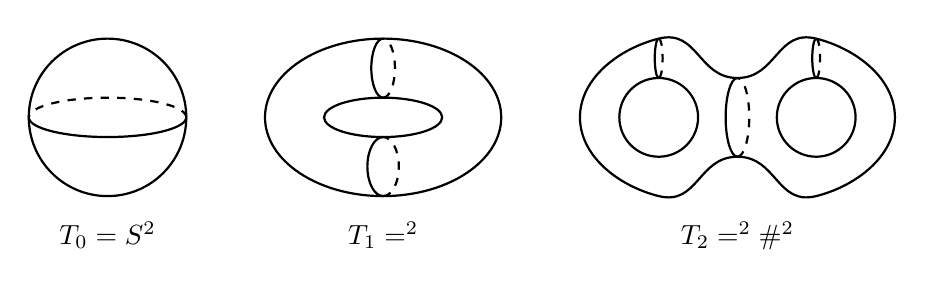
\begin{tikzpicture}
    % Sphère
    \draw[thick] (0,0) circle (1cm);
    \draw[thick] (-1,0) arc (180:360:1 and .25);
    \draw[thick,dashed] (1,0) arc (0:180:1 and .25);
    \node at (0,-1.2) [below] {$T_0=\mathbb S^2$};

    % Tore 
    \draw[thick] (3.5,0) ellipse (1.5cm and 1cm);
    \draw[thick] (3.5,0) ellipse (.75cm and .25cm);
    \draw[thick] (3.5,-1) arc (270:90:.2 and .375);
    \draw[thick,dashed] (3.5,-1) arc (-90:90:.2 and .375);
    \draw[thick] (3.5,.25) arc (270:90:.15 and .375);
    \draw[thick,dashed] (3.5,.25) arc (-90:90:.15 and .375);
    \node at (3.5,-1.2) [below] {$T_1=\T^2$};

    % Quadruble tore
    \node (p1) at (6,0) {};
    \node (p2) at (7,1) {};
    \node (p3) at (8,.5) {};
    \node (p4) at (9,1) {};
    \node (p5) at (10,0) {};
    \node (p6) at (9,-1) {};
    \node (p7) at (8,-.5) {};
    \node (p8) at (7,-1) {};
    \draw[thick] (7,0) circle (.5);
    \draw[thick] (9,0) circle (.5);
    \draw[thick] (8,-.5) arc (270:90:.15 and .5);
    \draw[thick,dashed] (8,-.5) arc (-90:90:.15 and .5);
    \draw[thick] (7,.5) arc (270:90:.05 and .25);
    \draw[thick,dashed] (7,.5) arc (-90:90:.05 and .25);
    \draw[thick] (9,.5) arc (270:90:.05 and .25);
    \draw[thick,dashed] (9,.5) arc (-90:90:.05 and .25);
    \path[thick,draw] plot [smooth cycle,tension=.9] coordinates {(p1) (p2) (p3) (p4) (p5) (p6) (p7) (p8)};
    \node at (8,-1.2) [below] {$T_2=\T^2\#\T^2$};
\end{tikzpicture}\\
    \textsc{Figure 4} – \textit{Illustration de $T_g$ pour les genres $0$, $1$ et $2$.}
\end{center}
